\documentclass[preprint,12pt,authoryear]{elsarticle}

\usepackage{amsmath,amssymb,booktabs,multirow,graphicx,lineno,url}
\usepackage[hidelinks]{hyperref}
\graphicspath{{figures/}}
\newcommand{\dt}{$\Delta T$}
\journal{Smart Health}

\begin{document}

\begin{frontmatter}

\title{Accuracy does not buy timing: a lead-time metric for stress
anticipation in mobile sensing}

\author{David Olutunde Daniel$^{1,2,*}$\\[6pt]
\normalfont
$^1$Department of Mathematical Sciences, The University of Texas at Dallas, Richardson, TX, USA\\
$^2$AT\&T Chief Data Office, Dallas, TX, USA\\
$^*$Corresponding author. Email: dod220001@utdallas.edu; dd0532@att.com}

%% ── Abstract ──────────────────────────────────────────────────────────────
\begin{abstract}
Machine learning systems for stress detection are evaluated almost
exclusively on whether they classify the current state correctly. They
are rarely evaluated on whether they detect a stress transition early
enough to support intervention --- the property that matters most for
deployment. We introduce \dt{}, the signed time between a detected
change point in a model's predicted-stress trajectory and the nearest
ground-truth stress onset, and measure it on StudentLife (smartphone
behavioural sensing). Our central finding is a null result with
practical consequences. Across three model configurations whose
micro-F1 spans 0.478 to 0.611, timing does not differ detectably: among
onsets matched in both models, paired mean \dt{} differences are at
most 2.2 hours and fall within a $\pm 6$-hour equivalence margin under
two one-sided tests (in fact within $\pm 4.5$ hours), and the median
\dt{} is zero for every configuration, against a spread of 28 to 30
hours. Against two null models, none of the three shows significantly
more anticipation than randomly timed change points produce under the
same matching rule (observed rates 23--27\%).
Models retrained to forecast one to three EMA responses ahead (median
gaps of 16 to 49 hours) lose no accuracy and keep a median \dt{} of
zero. On identical validation sequences, no statistically detectable
paired mean timing difference from the present-state models was found;
equivalence within $\pm 6$ hours was supported for five of six
comparisons and one remained inconclusive. A
temporally asymmetric training objective designed specifically to shift
\dt{} earlier also fails to move it, while incidentally improving
macro-F1 by 3.1 to 3.4 points.
We also report a methodological caution: the anticipation rate, a
natural summary statistic, can rise when the \dt{} distribution widens
without shifting earlier, and in our data it differs between models
whose medians and paired mean differences do not. Change points are
located retrospectively, so \dt{} measures temporal alignment, not
real-time warning lead. We conclude
that timing and accuracy are separable properties of a stress-prediction
model, that standard metrics are silent about the former, and that
systems intended to anticipate rather than react will require methods
that target timing directly.
\end{abstract}

\begin{keyword}
stress prediction \sep mobile sensing \sep anticipation \sep
change-point detection \sep reproducibility \sep digital health \sep
ecological momentary assessment
\end{keyword}

\end{frontmatter}

%% ──────────────────────────────────────────────────────────────────────────
\section{Introduction}
%% ──────────────────────────────────────────────────────────────────────────

Chronic and episodic stress contributes to a wide range of adverse health
outcomes, including cardiovascular disease, immune dysfunction, sleep
disruption, and elevated risk for mood and anxiety disorders
\citep{cohen1983,mcewen2007,chrousos2009}. The public health burden of
these downstream conditions has motivated a decade of work on stress
detection from continuous mobile and wearable sensing
\citep{wang2014,schmidt2018,sano2013,gjoreski2016}. The underlying
premise of that work is preventive: if a system can identify stress
early, intervention becomes possible before consolidation into a chronic
pattern or a physiological episode.

Predictive healthcare, as distinguished from reactive diagnosis, depends
on lead time. A model that identifies deterioration only after
symptomatic onset is useful for retrospective analysis; it is not useful
for preventive action. In cardiac monitoring, in glycaemic prediction,
and in early-warning scoring for sepsis
\citep{ebrahimzadeh2018,debois2022,henry2015,goldstein2017}, the interval between model
detection and clinical event is treated as a core evaluation quantity
alongside sensitivity and specificity. In stress prediction, no such
quantity exists.

The absence is consequential. Standard machine learning metrics ---
micro-F1, macro-F1, accuracy, area under the ROC curve --- are all
computed relative to per-window labels. Models with similar
classification scores can nevertheless differ substantially in
detection timing. These metrics do not directly quantify the interval
between a model's detected transition and the reported onset. For a
system whose stated purpose is to enable a timely response ---
suggesting a break, prompting a coping exercise, escalating to a
clinician --- that interval is what matters.

This paper introduces a measurement for the missing quantity, applies
it to the StudentLife smartphone-sensing dataset, and reports
what it shows. Models trained to predict the current label are not, of
course, designed to anticipate. The point of \dt{} is to make the
timing property measurable rather than assumed --- and then to test
directly whether it responds to the levers available to a system
designer: higher accuracy, personalisation, a timing-targeted
objective, or training the model to forecast ahead. \dt{} is defined as the signed time between a change
point in the model's own stress trajectory and the nearest
ground-truth stress onset. Negative values indicate the model detected
the transition before the person reported it --- anticipation. Positive
values indicate reactive detection.

The framework is deliberately model-agnostic. It requires only that the
model emit class probabilities over a temporally ordered evaluation set,
which every modern classifier does by default. It requires no changes
to model architecture, no additional annotation, and no retraining. It
sits alongside standard classification metrics as a complementary
measurement of lead time.

Our contributions to predictive healthcare research are as follows.

\begin{enumerate}

\item \textbf{A lead-time metric for stress anticipation.} \dt{}
formalises the notion of anticipation in a form directly comparable to
lead-time metrics used in other predictive-healthcare domains such as
cardiac arrhythmia forecasting, glycaemic prediction, and sepsis
early warning.

\item \textbf{An equivalence result across architectures.} Across
three model configurations spanning 13.3 points of micro-F1 on
StudentLife, paired mean \dt{} differences on onsets matched in both
models fall within a $\pm 6$-hour equivalence margin, with inference
from a bootstrap that resamples students. No configuration shows
significantly more anticipation than either of two chance-level null
models, and the pattern persists under a control for segmentation
sensitivity.

\item \textbf{Two anticipation-targeted interventions.} A temporally
asymmetric loss function constructed specifically to shift \dt{}
earlier does not shift it, producing instead an unrelated gain in
macro-F1. Retraining the models to forecast one to three EMA responses
ahead leaves classification accuracy unchanged, and on identical
validation sequences no statistically detectable paired mean timing
difference from the present-state models was found; equivalence within
$\pm 6$ hours was supported for five of six comparisons, and the
baseline at $h = 2$ remained inconclusive. Both results are informative
for the design of future intervention-oriented systems.

\item \textbf{A methodological caution.} The anticipation rate, a
natural summary statistic, can increase when the \dt{} distribution
widens without shifting. In our data it differs between models whose
medians and paired mean differences do not. We recommend that predictive-healthcare studies report the
median, interquartile range, and a distributional distance alongside
the anticipation rate.

\end{enumerate}

We also report an independent reproduction of the published baselines
we build on. That reproduction is a precondition for the rest of the
analysis rather than a contribution in itself, and we treat it
accordingly.

The findings have direct implications for the design and evaluation of
predictive-healthcare systems built on mobile and wearable sensing. If
lead time is fixed by the sensing modality and annotation protocol
rather than by the model, investment in classifier accuracy will not
by itself produce more clinically actionable systems. Progress will
require either (a) methods that explicitly target the timing property,
or (b) modifications to sensing and annotation infrastructure to
shorten the ground-truth delay itself.

%% ──────────────────────────────────────────────────────────────────────────
\section{Related work}
%% ──────────────────────────────────────────────────────────────────────────

\subsection{Stress detection from mobile and wearable sensing}

Passively collected smartphone signals predict self-reported stress
meaningfully above chance. Early work by
\citet{sano2013} demonstrated the feasibility of continuous stress
recognition using accelerometer, skin conductance, and phone usage
data. \citet{wang2014} extended this to a ten-week longitudinal
benchmark on 48 undergraduates at Dartmouth College, combining phone
sensing with daily ecological momentary assessment, and the resulting
dataset remains one of the most widely used public resources for
naturalistic stress and mental-health sensing. On the physiological
side, \citet{schmidt2018} introduced WESAD, a controlled multimodal
wearable dataset collected under the Trier Social Stress Test protocol,
spanning electrocardiogram, electrodermal activity, blood volume pulse,
electromyogram, skin temperature, respiration, and three-axis
acceleration from chest and wrist devices.

Across this literature, modelling individual differences consistently
improves performance, and personalisation schemes that condition on
subject identity or subject-level characteristics are common. Deep
learning approaches, particularly LSTM autoencoders and their
personalised extensions, have demonstrated strong results on these
tasks \citep{iflrepo,hovsepian2015,taylor2020}. Complementary work
using galvanic skin response and other physiological signals has
established the feasibility of stress pattern detection from wearable
sensors alone \citep{bakker2011,gjoreski2016}.

Instrumented self-report of stress is the standard ground truth in this
literature, with the Perceived Stress Scale
\citep{cohen1983} and daily ecological momentary assessment prompts the
two most common protocols. Both introduce delay between the underlying
physiological or behavioural signal and the recorded label; this delay
is one of the properties that a lead-time metric such as \dt{}
implicitly measures.

\subsection{Predictive healthcare and lead-time metrics}

Predictive-healthcare systems in adjacent domains are routinely
evaluated on how far in advance they detect events. Paroxysmal atrial fibrillation
predictors are evaluated on their ability to flag the interval
immediately preceding an episode \citep{ebrahimzadeh2018}. Sepsis early-warning scoring
systems are evaluated on the interval between prediction and clinical
onset \citep{henry2015,goldstein2017}. Continuous glucose monitoring
combined with machine learning is benchmarked at explicit prediction
horizons of 30 to 120 minutes, to enable preemptive dosing
decisions \citep{debois2022}. Across these domains,
lead time is measured directly, not inferred from classification
metrics.

Stress prediction has not adopted this practice. The absence is
sometimes attributed to the inherent difficulty of establishing a
precise onset timestamp for a self-reported subjective state.
Change-point detection provides an operational answer: rather than
require an externally validated onset, define the onset as the moment
the recorded label crosses a threshold and treat the model's own
stress trajectory as an independent observation whose alignment
with that moment can be measured. This is the approach we adopt.

\subsection{Temporal structure in health sensing}

Most work treats stress prediction as static classification: given a
window of sensor data, predict the label for that window. The temporal
dynamics, and in particular whether a model's internal state shifts
before the corresponding shift appears in self-report, have received
considerably less attention. The notion of an anticipation window is
implicit in work on affect forecasting and in the predictive-maintenance
literature more broadly \citep{lei2018}, but to our knowledge has not
been formalised as a directly measurable quantity for stress prediction
prior to this work.

\subsection{Change-point detection}

Change-point detection has an established history in physiological and
behavioural time series. The PELT algorithm \citep{killick2012} provides
an exact solution with linear expected computational cost under a broad
family of cost functions, which suits the relatively short per-subject
sequences typical of ecological momentary assessment studies. Related
methods based on dynamic programming \citep{jackson2005} and a broader
family of offline detection procedures are reviewed by
\citet{truong2020}. Our use of these methods differs from the standard
application: we apply change-point detection to the model's output
trajectory rather than to the input signal, converting a detection tool
into an instrument for measuring model behaviour.

\subsection{Reproducibility in machine learning for health}

Reproducibility difficulties are widely documented across machine
learning \citep{pineau2021}. Health applications face additional
obstacles from restricted data, privacy constraints, and the distance
between research prototypes and deployable systems
\citep{beam2018,futoma2020}. Our own experience during this work
reinforces a narrower point: configuration errors that produce
plausible-looking results are a distinct and under-discussed failure
mode, separate from the more commonly cited issues of hyperparameter
sensitivity and random seed variation. We document this in
Section~\ref{sec:repro}.

%% ──────────────────────────────────────────────────────────────────────────
\section{Data and models}
%% ──────────────────────────────────────────────────────────────────────────

\subsection{Dataset}

StudentLife \citep{wang2014} was conducted at Dartmouth College over a
ten-week academic term in spring 2012. Forty-eight undergraduate students
carried an instrumented Android phone that logged GPS traces, Wi-Fi
access points, accelerometer activity, ambient audio features, call and
message metadata, and application usage. Daily ecological momentary
assessment prompts collected self-reported stress on a five-point scale,
collapsed for this task into three classes: no or minimal stress, mild
stress, and high stress.

After the preprocessing supplied with the reference implementation,
1{,}175 labelled examples remain across 23 students, each with 14
normalised feature channels. The class distribution is 22.1\%,
43.4\%, and 34.5\% respectively; this imbalance depresses
macro-averaged F1 relative to micro-averaged F1 throughout.

Each example carries a compound key encoding subject identity and
observation time at hour resolution. This permits reconstruction of a
per-subject timeline directly from the evaluation set, without auxiliary
timestamp files, which is what makes the \dt{} computation possible on
this dataset.

\subsection{Model configurations}

We use the reference implementation released by the Information Fusion
Laboratory at the University of Massachusetts Amherst \citep{iflrepo}.
Three configurations are compared:

\begin{itemize}
\item \textbf{LSTM baseline.} The reference implementation's
\texttt{lstm} configuration: the LSTM autoencoder architecture without
personalisation, trained with the classification loss only (the
reconstruction term is switched off in this configuration, so the
decoder is not trained). All subjects share a single output head.
\item \textbf{Personalised, one branch.} The \texttt{calm\_net}
configuration: the same LSTM autoencoder trained with the
reconstruction term, per-subject output heads, and a single-branch
routing module.
\item \textbf{Personalised, three branches.} As above with a
three-branch routing module.
\end{itemize}

These are the configurations the reference implementation designates as
its baseline and its personalised models. They differ in two respects,
personalisation and the reconstruction term, so the accuracy gap
between them should not be attributed to personalisation alone. For
this paper what matters is that they are models of clearly different
accuracy trained on the same folds.

Personalisation operates through a subject-to-group mapping combined
with per-subject output layers held in a module dictionary keyed by
subject identifier.

\subsection{Training protocol}
\label{sec:protocol}

Ten repetitions of five-fold cross-validation, giving 50 folds in total,
with 200 epochs per fold. Folds are those of the reference
implementation: a deterministic stratified five-fold split at the
example level, stratified jointly by student and stress label. Every
student therefore contributes examples to both the training and the
validation partition of every fold. This is what makes per-subject
output heads usable at validation time, and it means the reported F1
measures within-subject generalisation to unseen days, not
generalisation to unseen individuals. Each student's validation
examples in a fold form a temporally sparse subsequence of that
student's timeline (about one fifth of their EMA responses), and it is
on this subsequence that \dt{} is computed. The split depends only on
the labels, so all configurations trained on the same data file share
identical folds; this is what makes the onset-paired comparisons of
Section~\ref{sec:paired} possible.

Following the reference implementation, each fold is summarised by its
peak validation micro-F1 over the 200 epochs, and the model outputs at
that epoch are the ones used for the \dt{} analysis. This rule is
applied identically to every configuration, including the asymmetric
and forecasting runs. Because the epoch is chosen on the validation
fold itself and there is no separate test set, the reported F1 values
are optimistic; we use them to rank configurations, as the reference
implementation does, and not as estimates of deployed accuracy. All models were retrained for this revision on NVIDIA A30 and H100
GPUs, one repetition (five folds) per job, with a distinct random seed
per repetition.

%% ──────────────────────────────────────────────────────────────────────────
\section{Reproduction}
\label{sec:repro}
%% ──────────────────────────────────────────────────────────────────────────

Both published baselines reproduce. Table~\ref{tab:repro} and
Figure~\ref{fig:f1} report the results.

\begin{table}[h]
\centering
\caption{Reproduction of published baselines on StudentLife. Mean and
standard deviation of micro-F1 across 50 folds (10 repetitions of
5-fold cross-validation), except the authors' released checkpoint,
which contains 5 folds. All configurations were retrained for this
revision; every result in Section~\ref{sec:results} derives from these
runs.}
\label{tab:repro}
\resizebox{\textwidth}{!}{%
\begin{tabular}{lcc}
\toprule
Configuration & Micro-F1 & Published target \\
\midrule
LSTM baseline & $0.4783 \pm 0.030$ & $\approx 0.47$ \\
Authors' released checkpoint & $0.5991$ & $\approx 0.60$ \\
Personalised, one branch & $0.6034 \pm 0.028$ & $\approx 0.60$ \\
Personalised, three branches & $0.6112 \pm 0.022$ & $\approx 0.60$ \\
\bottomrule
\end{tabular}}
\end{table}

\begin{figure}[htbp]
\centering
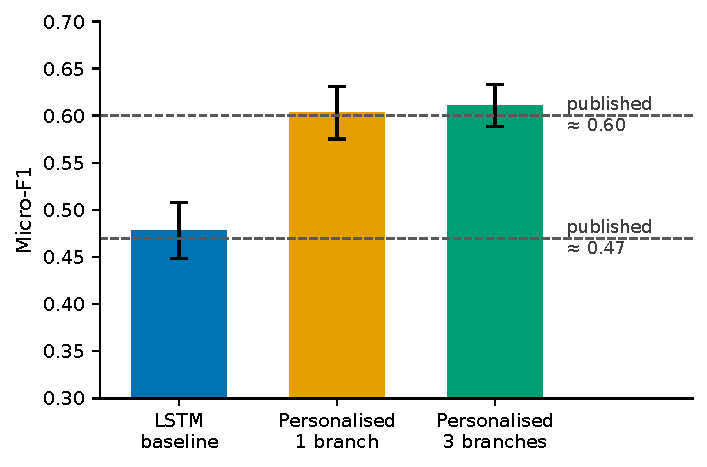
\includegraphics[width=0.75\textwidth]{fig1_f1_comparison.pdf}
\caption{Reproduction of published baselines. Error bars show one
standard deviation across 50 folds. Dashed lines mark the published
targets. Both targets are met.}
\label{fig:f1}
\end{figure}

Four independent lines of evidence confirm the personalised result: the
authors' released checkpoint (0.5991), two independently trained
configurations (0.6034 and 0.6112), and the originally published figure.

We note one methodological point that arose during this reproduction.
An earlier phase of this work concluded, incorrectly, that the
personalised model failed to reproduce its published performance. The
cause was a configuration error: the training entry point accepts six
positional arguments, of which the fifth selects the subject-to-group
mapping and the sixth is an unused output label. Three supposedly
distinct configurations had been run with the same value for the fifth
argument, varying only the sixth. They were the same model executed
three times, and the near-identical results they produced were
interpreted as a substantive finding.

\sloppy This failure mode deserves documentation because the resulting numbers
were entirely plausible. The fifth argument controls whether the model
uses a mapping that assigns all 23 subjects to a single group
(\texttt{all\_in\_one.pkl}, 718 bytes) or a mapping that assigns each
subject to its own group (\texttt{one\_for\_each.pkl}, 731 bytes).
Both files shipped with the repository. Personalisation is meaningless
under \texttt{all\_in\_one}: every subject shares one output head. All
results in this paper were produced after identifying and correcting
this error.

%% ──────────────────────────────────────────────────────────────────────────
\section{The \dt{} metric}
\label{sec:dt}
%% ──────────────────────────────────────────────────────────────────────────

We define the anticipation window as:

\begin{equation}
\Delta T = t_{\mathrm{model}} - t_{\mathrm{self\text{-}report}}
\label{eq:dt}
\end{equation}

where $t_{\mathrm{model}}$ is the timestamp of a change point in the
model's stress trajectory and $t_{\mathrm{self\text{-}report}}$ is
the timestamp of the nearest ground-truth stress onset within a matching
window. Negative \dt{} indicates anticipation; positive \dt{} indicates
reactive detection. The change points are located offline, using each
subject's complete validation trajectory, so \dt{} measures
retrospective temporal alignment between the model's trajectory and the
reported onsets. It is not the lead time of an alert that a deployed
system could have issued in real time; we return to this in
Section~\ref{sec:limits}.

\subsection{Pipeline}

\paragraph{Timeline reconstruction} The identifiers of each fold's
validation examples are stored with the fold's training record, so the
analysis reads them directly instead of reconstructing the split. Each
validation
example's compound key parses to a timestamp expressed as hours since a
fixed epoch.

\paragraph{Stress trajectory} For each example we compute the
per-row softmax $\mathbf{p}_t = (p_t^{(0)}, p_t^{(1)}, p_t^{(2)})$ over
the three ordered stress classes and form the expected stress level
\begin{equation}
s_t = \sum_{c=0}^{2} c \, p_t^{(c)} \in [0, 2],
\label{eq:stress}
\end{equation}
which increases monotonically with the probability mass placed on
higher stress and therefore represents stress directly. Examples are
grouped by subject and sorted chronologically. The originally submitted
analysis used the maximum class probability $\max_c p_t^{(c)}$, which
measures model certainty rather than stress; we retain it only as a
sensitivity analysis (\ref{app:maxprob}).

\paragraph{Change-point detection} We apply PELT \citep{killick2012}
with a radial basis function cost to each subject's stress
trajectory, using a minimum segment length of two examples and a
candidate grid of every example (\texttt{jump}~$=1$). The penalty was calibrated by scanning
$\{0.5, 1.0, 2.0, 5.0\}$ on a representative fold; a penalty of 1.0
was selected as neither over- nor under-segmenting.

\paragraph{Matching} Ground-truth stress onsets are upward transitions
in the chronological label sequence. Each detected change point is
matched to its nearest onset within a 72-hour window, and the signed difference recorded. Subjects contributing fewer than five examples to
a fold are excluded.

\subsection{An implementation detail worth recording}

The \texttt{ruptures} library \citep{truong2020} returns a list of
change-point indices whose final element equals the length of the
signal, functioning as a terminating sentinel rather than a detected
change. Retaining that element introduces one spurious change point per
subject, positioned at the end of the series and therefore
systematically late.

In our data this single error shifted the measured anticipation rate
from 29.3\% to 12.8\%. A second library default deserves the same
warning: \texttt{ruptures} evaluates candidate change points only on a
grid of every fifth sample unless \texttt{jump} is set explicitly. On
StudentLife validation subsequences of roughly ten examples per
subject, the default leaves only one or two admissible positions. The
originally submitted analysis used this default; all results in this
revision use \texttt{jump}~$=1$, and \ref{app:maxprob}
reports the submitted configuration for comparison: the coarse grid
admits roughly a third as many matched pairs (332--420 against
914--1120) and moves the median \dt{} from 0 to between $+4.0$ and
$+5.5$ hours. We report it because the resulting figure was
plausible and, taken at face value, supported a substantive but
incorrect conclusion.

%% ──────────────────────────────────────────────────────────────────────────
\section{Results}
\label{sec:results}
%% ──────────────────────────────────────────────────────────────────────────

\subsection{\dt{} under a fixed penalty}
\label{sec:fixedpen}

Table~\ref{tab:pelt} and Figures~\ref{fig:hist} and~\ref{fig:kde}
report \dt{} for the three configurations.

\begin{table}[h]
\centering
\caption{\dt{} statistics under PELT with penalty 1.0, pooled over ten
repetitions per configuration. The anticipation rate is the proportion
of matched pairs with $\Delta T < 0$, reported pooled and as mean $\pm$
standard deviation across the ten repetitions; ties ($\Delta T = 0$,
also shown) count as reactive. All time values are in hours.}
\label{tab:pelt}
\small
\resizebox{\textwidth}{!}{%
\begin{tabular}{lcccccccc}
\toprule
Configuration & F1 & $N$ & Mean & Median & Std & IQR & $\Delta T = 0$ & Anticipation \\
\midrule
LSTM baseline        & 0.478 & 1120 & $+8.40$ & $0$ & 27.8 & 24.0 & 35.3\% & 22.8\% ($22.8 \pm 2.1$) \\
Personalised, 1 br.  & 0.603 & 1064 & $+6.97$ & $0$ & 30.4 & 30.0 & 32.8\% & 26.4\% ($26.4 \pm 2.7$) \\
Personalised, 3 br.  & 0.611 & 914  & $+6.65$ & $0$ & 30.0 & 29.0 & 32.6\% & 26.6\% ($26.7 \pm 4.8$) \\
\bottomrule
\end{tabular}}
\end{table}

\begin{figure}[htbp]
\centering
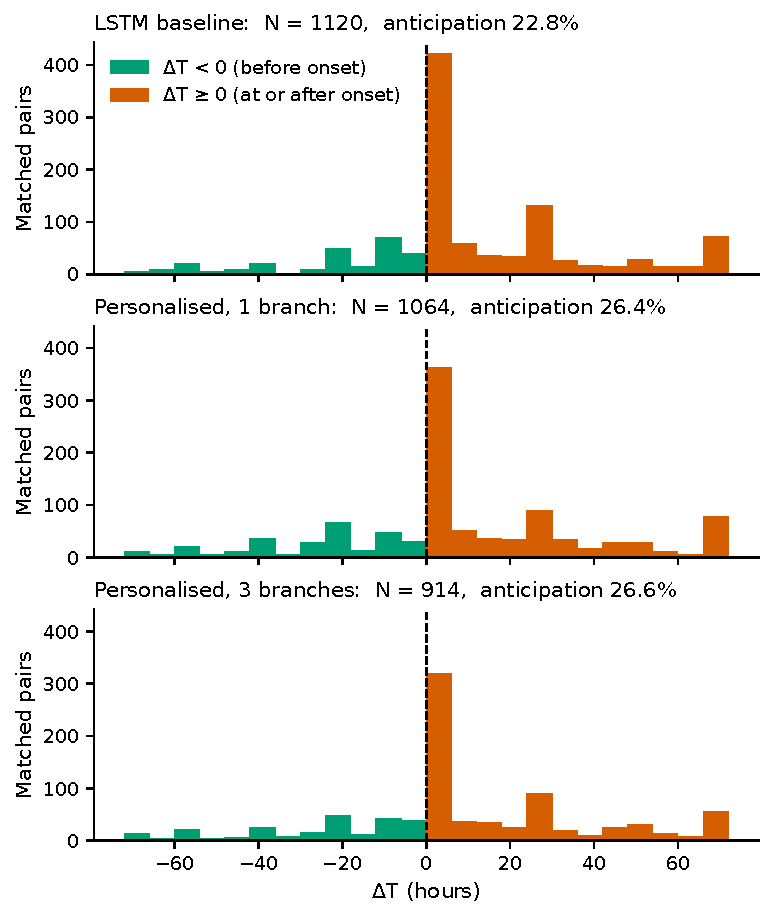
\includegraphics[width=0.8\textwidth]{fig2_delta_t_hist.pdf}
\caption{\dt{} distributions for the three configurations. Green bars
indicate anticipated transitions ($\Delta T < 0$); orange bars indicate
reactive detections ($\Delta T \geq 0$). Dashed vertical lines mark the
median (0 hours in all three panels). Panel annotations are generated
from the same records as Table~\ref{tab:pelt}. The three panels are
visually near-identical despite a 13.3-point spread in micro-F1.}
\label{fig:hist}
\end{figure}

\begin{figure}[htbp]
\centering
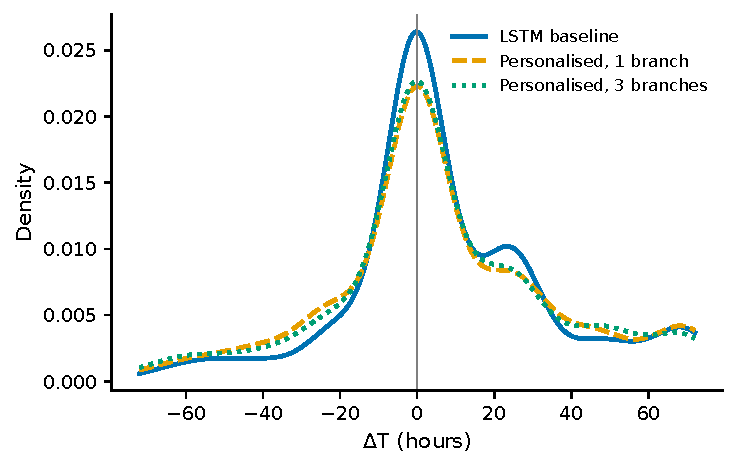
\includegraphics[width=0.75\textwidth]{fig3_delta_t_kde.pdf}
\caption{Kernel density estimates of the three \dt{} distributions.
The curves nearly coincide despite a 13.3-point spread in micro-F1.}
\label{fig:kde}
\end{figure}

As a descriptive summary, the pairwise Wasserstein distances between
the pooled \dt{} distributions are 2.65, 2.45, and 0.85 hours
(baseline--1-branch, baseline--3-branch, 1-branch--3-branch), with
Mann-Whitney $p$ values of 0.217, 0.188, and 0.917. Because matched
pairs that share an onset or a subject are not independent, we do not
treat these pooled tests as inferential; the paired analysis of
Section~\ref{sec:paired} is the inferential comparison. We note also
that the sample sizes differ across configurations (1120, 1064, 914),
indicating that the fixed penalty segments each model's stress
trajectory at a different effective sensitivity; Section~\ref{sec:fixedk}
removes this confound.

\subsection{Null models: what chance timing produces}
\label{sec:nulls}

A \dt{} distribution is only interpretable against what the same
matching rule yields when the change points carry no information about
the onsets. We constructed two null models, each with 1{,}000 draws per
configuration.

\paragraph{Random change points} Within each subject-fold trajectory,
the detected change points are replaced by the same number of positions
drawn uniformly at random, and the matching is repeated.

\paragraph{Shifted labels} Each subject's label sequence is circularly
shifted by a random offset, preserving its autocorrelation and onset
count while breaking any alignment with the model trajectory; the
model's actual change points are then matched against the shifted
onsets.

We compare three statistics: the anticipation rate, the median \dt{},
and an alignment statistic --- the proportion of change points landing
within $\pm 24$ hours of an onset. Table~\ref{tab:nulls} and
Figure~\ref{fig:nulls} report the results.

\begin{table}[h]
\centering
\caption{Observed statistics against the two null models (mean and 95\%
interval over 1{,}000 draws). $p_{\mathrm{ant}}$ is the proportion of
null draws with an anticipation rate at or below the observed one;
$p_{\mathrm{align}}$ the proportion with alignment at or above the
observed one. No configuration's anticipation rate is significantly
above either null; alignment is above the random-change-point null only
for the baseline, and no configuration is above the shifted-label null.}
\label{tab:nulls}
\small
\resizebox{\textwidth}{!}{%
\begin{tabular}{llccc}
\toprule
 & & Baseline & Pers., 1 br. & Pers., 3 br. \\
\midrule
Observed & Anticipation (\%) & 22.8 & 26.4 & 26.6 \\
         & Within $\pm24$ h of onset (\%) & 51.0 & 46.1 & 47.4 \\
\midrule
Random change points & Anticipation (\%) & 26.2 [23.8, 28.6] & 25.9 [23.6, 28.1] & 25.9 [23.5, 28.4] \\
 & \quad $p_{\mathrm{ant}}$ & $<0.01$ & 0.67 & 0.70 \\
 & Within $\pm24$ h (\%) & 46.5 [44.5, 48.5] & 46.2 [44.1, 48.2] & 45.5 [43.2, 47.9] \\
 & \quad $p_{\mathrm{align}}$ & $<0.01$ & 0.57 & 0.06 \\
\midrule
Shifted labels & Anticipation (\%) & 40.0 [37.6, 42.3] & 39.7 [37.0, 42.3] & 38.5 [35.8, 41.4] \\
 & \quad $p_{\mathrm{ant}}$ & $<0.01$ & $<0.01$ & $<0.01$ \\
 & Within $\pm24$ h (\%) & 49.6 [47.8, 51.4] & 51.2 [49.2, 53.1] & 50.3 [48.0, 52.3] \\
 & \quad $p_{\mathrm{align}}$ & 0.07 & 1.00 & 1.00 \\
\bottomrule
\end{tabular}}
\end{table}

\begin{figure}[htbp]
\centering
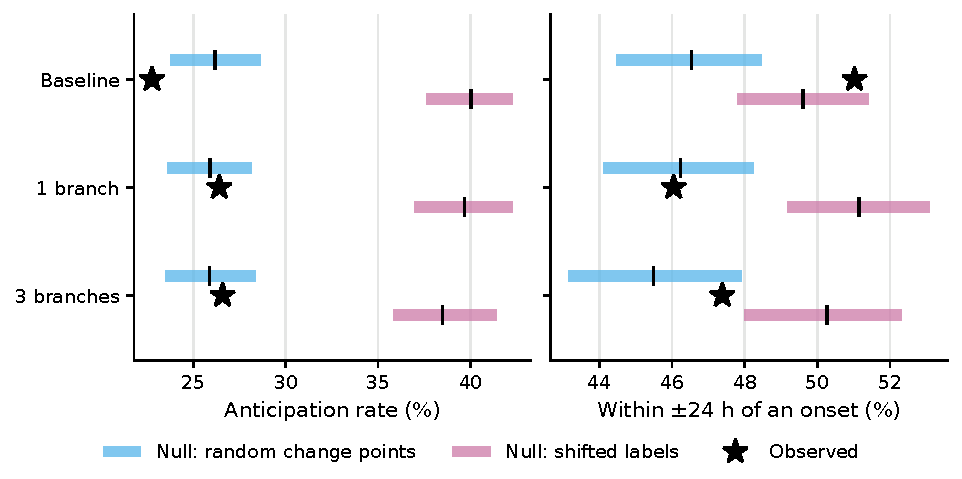
\includegraphics[width=\textwidth]{fig7_null_models.pdf}
\caption{Observed anticipation rate (left) and onset alignment (right)
against the two null models. Stars are the observed values; bars are
the 95\% intervals of each null over 1{,}000 draws, with the null mean
marked. No observed anticipation rate is significantly above either
null.}
\label{fig:nulls}
\end{figure}

Three facts follow. First, no configuration shows significantly more
anticipation than randomly timed change points produce under the same
matching rule. The personalised models' rates (26.4\% and 26.6\%) sit
just above the random-change-point mean of 25.9\% and well inside its
95\% interval (67\% and 70\% of null draws fall at or below them); the baseline's rate (22.8\%) is
significantly \emph{below} it. An anticipation rate near 26\% is
therefore what this matching rule yields without any timing information,
and is not by itself evidence of early warning. Second, against the
shifted-label null, whose anticipation rate is 38--40\%, every observed
rate is far lower ($p < 0.01$): relative to onsets placed at unrelated
positions, the models' change points fall before an onset much less
often, which is the pattern expected of detection at or after the
onset. Third, the alignment statistic gives a mixed picture. The
baseline's change points fall within $\pm 24$ hours of an onset more
often than random change points do (51.0\% against 46.5\%,
$p < 0.01$), but not more often than under shifted labels ($p = 0.07$);
neither personalised model is above either null. The two nulls give
different reference values for the same statistic (26\% and 39\%
anticipation), which is itself a reason not to interpret an
anticipation rate without stating the reference. In summary, no
configuration showed significantly greater anticipation than either
null; the baseline showed greater onset alignment than the
random-change-point null, but not than the shifted-label null.

\subsection{Onset-paired equivalence between models}
\label{sec:paired}

Because every configuration shares identical folds
(Section~\ref{sec:protocol}), each ground-truth onset can be matched across models.
For each onset we take the \dt{} of each model's nearest change point
within the 72-hour window (median across the ten repetitions) and
compare models on the paired differences. An onset enters a pair only
if both models have a change point within the window in at least one
repetition; onsets matched in one model but not the other are excluded
from that pair, so the analysis concerns onsets that both models
respond to.

All inference is from a bootstrap that resamples \emph{students} with
replacement (2{,}000 draws) and recomputes the paired mean difference,
so that multiple onsets from one student, and the ten repetitions,
are not treated as independent. The confidence intervals are bootstrap
percentile intervals. For equivalence we use a margin of $\pm 6$ hours,
a quarter of the daily EMA cycle and the smallest advance we consider
actionable for a same-day intervention. The margin was fixed when the
revision analysis was designed, before the models were retrained and
before any result in this section was computed. The two one-sided
tests (TOST) are carried out on the same student-level bootstrap
distribution: the TOST $p$ value is the larger of the proportions of
bootstrap means at or beyond each margin, and equivalence at the 5\%
level corresponds to the 90\% interval lying inside the margin. Because
a reader may prefer a different margin, we also report the smallest
margin at which equivalence holds. We additionally report an
onset-level Wilcoxon signed-rank $p$ value as a description only: it
treats onsets as independent and should not be read as an inferential
result.

The tested quantity is the \emph{mean} paired difference. The analysis
does not establish that the \dt{} distributions have the same shape,
tails, or anticipation rate; those are described in
Sections~\ref{sec:fixedpen} and~\ref{sec:antrate}.

\begin{table}[h]
\centering
\caption{Onset-paired comparisons of \dt{} between models. The paired
difference is row model minus column model, in hours, with 95\%
student-clustered bootstrap confidence intervals. Equivalence is
assessed by TOST at the pre-specified $\pm 6$-hour margin; the final
column gives the smallest margin at which equivalence holds (the larger
absolute bound of the 90\% CI). The TOST $p$ value and the intervals
come from the student-level bootstrap; the Wilcoxon $p$ value is
onset-level and descriptive.}
\label{tab:paired}
\small
\resizebox{\textwidth}{!}{%
\begin{tabular}{lcccccc}
\toprule
Pair & Onsets & Mean diff.\ [95\% CI] & Wilcoxon $p$ & TOST $p$ & Equivalent at $\pm6$ h & Smallest margin \\
\midrule
Baseline vs.\ 1 br.   & 163 & $+2.16$ [$-0.88$, $+5.10$] & 0.509 & 0.005 & yes & 4.5 h \\
Baseline vs.\ 3 br.   & 166 & $+0.43$ [$-3.03$, $+3.73$] & 0.832 & $<0.001$ & yes & 3.3 h \\
1 br.\ vs.\ 3 br.     & 173 & $-0.97$ [$-3.14$, $+1.29$] & 0.086 & $<0.001$ & yes & 2.8 h \\
\bottomrule
\end{tabular}}
\end{table}

\begin{figure}[htbp]
\centering
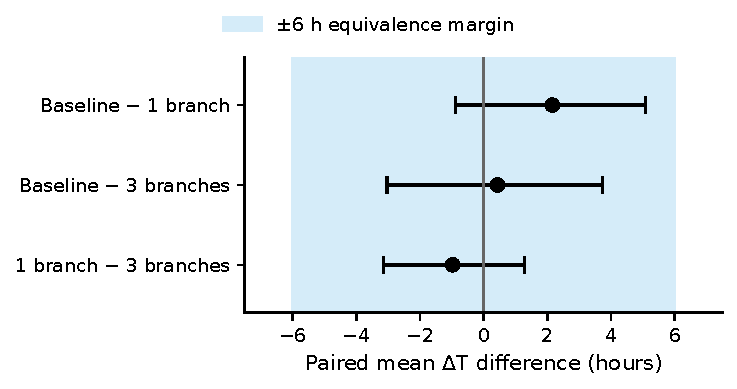
\includegraphics[width=0.75\textwidth]{fig4_paired_differences.pdf}
\caption{Onset-paired mean \dt{} differences between models with 95\%
student-clustered bootstrap confidence intervals, against the
pre-specified $\pm 6$-hour equivalence margin (shaded). Every interval
lies well inside the margin.}
\label{fig:paired}
\end{figure}

For all three pairs the paired mean difference is within the
$\pm 6$-hour margin, and in fact within 4.5, 3.3, and 2.8 hours
(Table~\ref{tab:paired}, Figure~\ref{fig:paired}). Against a
within-model \dt{} spread of roughly 28 hours, mean between-model
shifts larger than five hours are ruled out at the 90\% level for
every pair. This is a bound on the mean shift among onsets matched in
both models, which is a stronger statement than a failure to detect a
difference but a narrower one than equivalence of the distributions.

\subsection{Controlling for segmentation sensitivity}
\label{sec:fixedk}

To remove the sample-size confound noted in Section~\ref{sec:fixedpen} we repeated the
analysis using dynamic-programming segmentation \citep{jackson2005}
with a fixed number of change points per subject, sweeping
$k \in \{1, 2, 3\}$. Under this scheme every configuration produces
exactly $k$ change points for every subject.

\begin{table}[h]
\centering
\caption{\dt{} with segmentation granularity held constant. Every
configuration has exactly $k$ change points per subject; the number of
matched pairs $N$ (change points with an onset inside the window)
becomes similar across configurations at every $k$. The
anticipation rate is the repetition mean $\pm$ SD; the median \dt{} is
0 hours in every cell. Time values in hours.}
\label{tab:nbkps}
\small
\begin{tabular}{llcccc}
\toprule
$k$ & Configuration & $N$ & Mean & Std & Anticipation \\
\midrule
\multirow{3}{*}{1}
 & LSTM baseline       & 757  & $+7.48$ & 29.2 & $25.0 \pm 4.0$\% \\
 & Personalised, 1 br. & 763  & $+8.04$ & 30.8 & $22.9 \pm 4.3$\% \\
 & Personalised, 3 br. & 754  & $+6.40$ & 30.2 & $23.5 \pm 4.6$\% \\
\midrule
\multirow{3}{*}{2}
 & LSTM baseline       & 1469 & $+8.35$ & 27.1 & $20.6 \pm 1.7$\% \\
 & Personalised, 1 br. & 1477 & $+7.06$ & 29.3 & $22.7 \pm 2.4$\% \\
 & Personalised, 3 br. & 1479 & $+6.91$ & 29.8 & $23.4 \pm 3.6$\% \\
\midrule
\multirow{3}{*}{3}
 & LSTM baseline       & 2194 & $+7.03$ & 27.9 & $22.6 \pm 1.4$\% \\
 & Personalised, 1 br. & 2184 & $+7.60$ & 29.3 & $21.4 \pm 2.1$\% \\
 & Personalised, 3 br. & 2160 & $+7.04$ & 29.3 & $22.5 \pm 2.4$\% \\
\bottomrule
\end{tabular}
\end{table}

\begin{figure}[htbp]
\centering
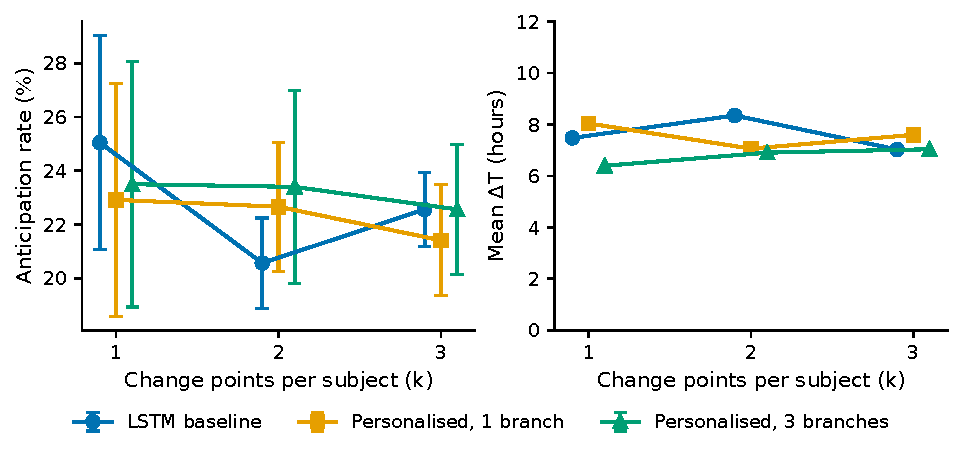
\includegraphics[width=\textwidth]{fig5_fixed_k.pdf}
\caption{Invariance under controlled segmentation. Left: anticipation
rates with standard deviation across repetitions, at each granularity.
Right: mean \dt{} (hours); the median is 0 hours for every
configuration at every granularity.}
\label{fig:nbkps}
\end{figure}

With the number of detected change points held equal, the number of
matched pairs becomes similar across configurations at every
granularity (754--763 at $k=1$, against 914--1120 under the fixed
penalty; Table~\ref{tab:nbkps}). This is consistent with the
fixed-penalty differences in $N$ arising from the penalty interacting
with differently shaped stress trajectories. The anticipation rates remain within
a five-point band (20.6--25.0\%) with overlapping repetition spreads,
and the median \dt{} is 0 hours in every cell. These are descriptive
summaries; the inferential comparison is the paired analysis of
Section~\ref{sec:paired}.

\subsection{On the anticipation rate as a summary statistic}
\label{sec:antrate}

The anticipation rate is the proportion of \dt{} values below zero. It
is an intuitive summary, and our data show two ways in which it can
mislead when reported alone.

First, it can differ between models whose central timing does not. The
per-repetition anticipation rates of the baseline and the
single-branch model differ ($22.8 \pm 2.1$\% against
$26.4 \pm 2.7$\%; two-sample $t$-test $p = 0.003$, and $p = 0.031$ for
baseline against three branches; descriptive, since repetitions share
folds). That difference in the rate is real. What it does not show is
a shift in timing: all three medians are 0 hours, and the paired mean
difference is bounded within 4.5 hours (Section~\ref{sec:paired}). The
personalised models' interquartile ranges are a quarter wider than the
baseline's (30 and 29 against 24 hours), so more of their mass lies on
both sides of zero. A proportion below a threshold can increase when a
distribution widens without moving, although it need not: widening a
distribution that is symmetric about zero leaves the proportion
unchanged. A higher anticipation rate should therefore not be read as
earlier detection unless the median or mean has moved with it.

Second, the rate has no meaning without a reference. The higher
personalised rates are not significantly above what random change
points give, and the two null models of Section~\ref{sec:nulls}
themselves differ by 13 points.

We recommend that studies using threshold-crossing summary statistics
of this kind report the median, interquartile range, a paired or
distributional comparison, and a chance-level null alongside them.

\subsection{A targeted training objective}

If \dt{} does not respond to architectural changes, it may respond to
the training objective. We implemented a temporally asymmetric loss that
upweights examples preceding a stress onset and downweights those
following it, with the explicit intent of shifting detections earlier.

\paragraph{Onsets} For each training subject $u$, examples are sorted
by timestamp $\tau_{u,1} < \dots < \tau_{u,n_u}$ (hours). A training
onset is any index $j \ge 2$ with $y_{u,j} > y_{u,j-1}$, giving the
onset set $\mathcal{O}_u = \{\tau_{u,j}\}$. Onsets are computed from
training labels only; validation labels are never used.

\paragraph{Weights} For example $i$ of subject $u$ with timestamp
$\tau_i$, let $o_i = \arg\min_{o \in \mathcal{O}_u} |\tau_i - o|$ (if
two onsets are equally near, the earlier one is used) and
$g_i = \tau_i - o_i$. With asymmetry strength $\lambda \ge 0$ and a
temporal window $H = 72$~h (equal to the \dt{} matching window),
\begin{equation}
w_i =
\begin{cases}
1 + \lambda, & -H \le g_i < 0 \quad \text{(pre-onset)},\\
(1 + \lambda)^{-1}, & 0 \le g_i \le H \quad \text{(onset and post-onset)},\\
1, & |g_i| > H \ \text{or}\ \mathcal{O}_u = \varnothing .
\end{cases}
\label{eq:asymw}
\end{equation}
$\lambda = 0$ recovers the standard objective; the pre/post weight
ratio is $(1+\lambda)^2$, i.e.\ 2.25 at $\lambda = 0.5$ and 4 at
$\lambda = 1$. Weights are fixed before training and are not
renormalised.

\paragraph{Objective} For a mini-batch $\mathcal{B}$, the
classification term is
\begin{equation}
\mathcal{L}_{\mathrm{cls}} = \frac{\beta}{|\mathcal{B}|}
\sum_{i \in \mathcal{B}} w_i \, \kappa_{y_i}
\left(-\log p_i^{(y_i)}\right),
\label{eq:asymloss}
\end{equation}
where $\kappa = (0.6456, 0.5635, 1.0000)$ are the reference
implementation's class weights for the three stress classes and
$\beta = 1$ is its classification-loss coefficient. The mini-batch size
is 1, as in the reference implementation. The total loss is
$\mathcal{L} = \alpha \mathcal{L}_{\mathrm{rec}} + \mathcal{L}_{\mathrm{cls}}$,
where $\mathcal{L}_{\mathrm{rec}}$ is the autoencoder reconstruction
term (L1, summed over elements) with $\alpha = 10^{-4}$. The asymmetric
objective was tested on the LSTM baseline configuration, in which the
reconstruction term is switched off, so for these runs
$\mathcal{L} = \mathcal{L}_{\mathrm{cls}}$. The temporal weights apply
to the training loss only. The epoch is selected by peak validation
micro-F1, exactly as for the symmetric baseline, so the two differ only
in the training objective.

\begin{table}[h]
\centering
\caption{\dt{} under a temporally asymmetric training objective at two
strengths ($\lambda$, Eq.~\ref{eq:asymw}). The objective did not shift
the anticipation window. The Mann-Whitney test and the onset-paired
mean difference (with 95\% student-clustered bootstrap CI, in hours)
are both against the symmetric baseline; medians are 0 hours
throughout. Macro-F1 is mean $\pm$ SD over 50 folds.}
\label{tab:asym}
\small
\resizebox{\textwidth}{!}{%
\begin{tabular}{lcccccc}
\toprule
Configuration & $N$ & Mean \dt{} (h) & Anticipation & MW $p$ & Paired $\Delta$ [95\% CI] & Macro-F1 \\
\midrule
Symmetric baseline          & 1120 & $+8.40$ & 22.8\% & ---   & --- & $0.332 \pm 0.044$ \\
Asymmetric, $\lambda = 0.5$ & 1108 & $+8.04$ & 24.6\% & 0.783 & $-0.13$ [$-2.73$, $+2.86$] & $0.366 \pm 0.046$ \\
Asymmetric, $\lambda = 1.0$ & 1124 & $+8.22$ & 23.3\% & 0.940 & $-1.78$ [$-5.26$, $+0.95$] & $0.363 \pm 0.056$ \\
\bottomrule
\end{tabular}}
\end{table}

\begin{figure}[htbp]
\centering
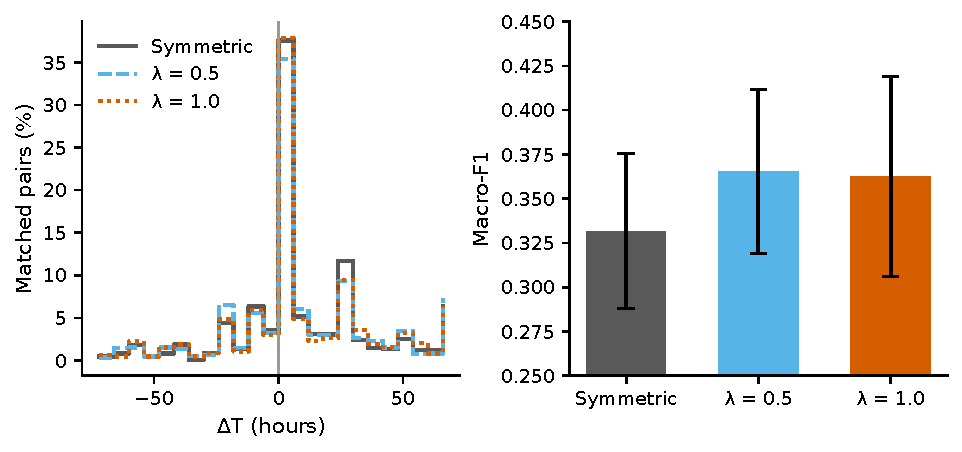
\includegraphics[width=0.85\textwidth]{fig6_asymmetric_loss.pdf}
\caption{A temporally asymmetric objective constructed to shift \dt{}
earlier does not do so at either strength tested (left: the three
\dt{} distributions, in 6-hour bins, nearly coincide).
The side effect, a macro-F1 improvement (right; error bars one SD
across 50 folds), is not the intended outcome.}
\label{fig:asym}
\end{figure}

The objective did not move \dt{} (Table~\ref{tab:asym},
Figure~\ref{fig:asym}): the Mann-Whitney $p$ values are 0.78 and 0.94,
and the onset-paired differences are $-0.13$ and $-1.78$ hours with
confidence intervals comfortably inside the $\pm 6$-hour equivalence
margin. It did produce a side effect: macro-F1 improved by
3.4 points at $\lambda = 0.5$ and 3.1 points at $\lambda = 1.0$
(fold-paired Wilcoxon signed-rank $p = 0.002$ and $p = 0.010$;
descriptive, since folds are shared across repetitions), at the cost of
a small drop in micro-F1 (0.455 and 0.467 against 0.478). A macro-F1
gain alongside a micro-F1 loss is the pattern expected if the weighting
shifted predictions toward the less frequent classes, and we interpret
it that way, but we did not record per-class scores and so cannot
confirm the mechanism. This is a real result, but not the one the
experiment was designed to produce.

\subsection{Training the models to forecast}
\label{sec:horizon}

A natural objection to everything above is that models trained to
predict the \emph{current} label have no reason to anticipate, so the
invariance is unsurprising. We accept the premise and test the obvious
remedy: retrain the models to predict the \emph{future} label. For
horizon $h \in \{1, 2, 3\}$, each training example's label is replaced
by the same student's $h$-th next EMA response (the last $h$ examples
per student are dropped), and the baseline and three-branch models are
retrained from scratch (5 repetitions $\times$ 5 folds per horizon).
The median time gap to the target response is 16, 30, and 49 hours at
$h = 1, 2, 3$. \dt{} is still measured against the current-label
onsets, so a model that truly anticipates by its trained horizon would
push the \dt{} distribution strongly negative.

\begin{table}[h]
\centering
\caption{Prediction-horizon experiment: accuracy and matched pairs.
Micro-F1 is mean $\pm$ SD over 25 folds (5 repetitions); $h = 0$ is the
main 50-fold run. The gap is the median time between an example and its
target label. $N$ is the number of matched pairs; \dt{} is computed
against current-label onsets and its median is 0 hours in every row.}
\label{tab:horizon}
\begin{tabular}{llccc}
\toprule
Configuration & $h$ & Gap (h) & Micro-F1 & $N$ \\
\midrule
\multirow{4}{*}{LSTM baseline}
 & 0 & ---  & $0.478 \pm 0.030$ & 1120 \\
 & 1 & 16   & $0.478 \pm 0.037$ & 618  \\
 & 2 & 30   & $0.482 \pm 0.032$ & 541  \\
 & 3 & 49   & $0.490 \pm 0.030$ & 532  \\
\midrule
\multirow{4}{*}{Personalised, 3 branches}
 & 0 & ---  & $0.611 \pm 0.022$ & 914  \\
 & 1 & 16   & $0.609 \pm 0.019$ & 526  \\
 & 2 & 30   & $0.610 \pm 0.014$ & 478  \\
 & 3 & 49   & $0.626 \pm 0.021$ & 494  \\
\bottomrule
\end{tabular}
\end{table}

\begin{table}[h]
\centering
\caption{Prediction-horizon experiment: timing on each run's own
validation sequences. Brackets after the observed values are 95\%
intervals from a bootstrap that resamples students. The null is the
random-change-point null for the same sequences (mean and 95\% interval
over 1{,}000 draws); $p$ is the proportion of null draws at or above
the observed rate, uncorrected for the six horizon tests. Rows with
different $h$ use different validation sequences and are not directly
comparable; Table~\ref{tab:horizondiff} gives the controlled
comparison.}
\label{tab:horizonnull}
\small
\resizebox{\textwidth}{!}{%
\begin{tabular}{llcccc}
\toprule
Configuration & $h$ & Mean \dt{} (h) & Anticipation (\%) & Null anticipation (\%) & $p$ \\
\midrule
\multirow{4}{*}{LSTM baseline}
 & 0 & $+8.4$ [$+4.3$, $+13.8$] & 22.8 [14.9, 30.0] & 26.2 [23.8, 28.8] & 1.00 \\
 & 1 & $+4.3$ [$+0.8$, $+8.6$]  & 28.3 [22.6, 33.3] & 29.3 [26.1, 32.5] & 0.70 \\
 & 2 & $+3.6$ [$+0.3$, $+7.7$]  & 32.7 [22.5, 40.5] & 28.9 [25.4, 32.4] & 0.02 \\
 & 3 & $+3.3$ [$-0.7$, $+7.7$]  & 34.2 [26.7, 40.3] & 31.5 [27.8, 35.4] & 0.08 \\
\midrule
\multirow{4}{*}{Personalised, 3 br.}
 & 0 & $+6.7$ [$+1.4$, $+12.4$] & 26.6 [18.3, 34.2] & 25.9 [23.3, 28.6] & 0.32 \\
 & 1 & $+3.8$ [$+0.2$, $+8.4$]  & 32.1 [25.1, 38.5] & 28.2 [24.9, 31.8] & 0.01 \\
 & 2 & $+1.3$ [$-2.5$, $+5.1$]  & 33.3 [26.0, 40.7] & 29.8 [26.0, 33.7] & 0.04 \\
 & 3 & $+0.6$ [$-3.3$, $+4.4$]  & 30.6 [23.2, 37.4] & 31.0 [27.3, 34.8] & 0.57 \\
\bottomrule
\end{tabular}}
\end{table}

\begin{table}[h]
\centering
\caption{Forecast-trained against present-state models on identical
validation sequences. For each forecast run, the present-state
($h = 0$) model's out-of-fold predictions for the same examples are
assembled into the same sequences and analysed in the same way. The
paired difference is forecast minus present, per onset matched in both
(median across repetitions), with a 95\% interval from a bootstrap that
resamples students; the last column states whether the 90\% interval
lies inside the $\pm 6$-hour margin.}
\label{tab:horizondiff}
\resizebox{\textwidth}{!}{%
\begin{tabular}{llccccccc}
\toprule
 & & \multicolumn{2}{c}{Mean \dt{} (h)} & \multicolumn{2}{c}{Anticipation (\%)} & & & \\
\cmidrule(lr){3-4}\cmidrule(lr){5-6}
Configuration & $h$ & Forecast & Present & Forecast & Present & Onsets & Paired difference (h) [95\% CI] & Within $\pm 6$ h \\
\midrule
\multirow{3}{*}{LSTM baseline}
 & 1 & $+4.3$ & $+3.4$ & 28.3 & 29.1 & 165 & $+1.1$ [$-2.2$, $+4.1$] & yes \\
 & 2 & $+3.6$ & $+4.0$ & 32.7 & 33.2 & 170 & $+2.0$ [$-5.2$, $+8.0$] & no  \\
 & 3 & $+3.3$ & $+0.7$ & 34.2 & 36.4 & 160 & $-0.6$ [$-5.7$, $+3.4$] & yes \\
\midrule
\multirow{3}{*}{Personalised, 3 br.}
 & 1 & $+3.8$ & $+1.6$ & 32.1 & 35.4 & 171 & $+1.9$ [$-1.9$, $+5.9$] & yes \\
 & 2 & $+1.3$ & $+4.0$ & 33.3 & 30.9 & 164 & $-1.0$ [$-5.5$, $+3.4$] & yes \\
 & 3 & $+0.6$ & $+3.8$ & 30.6 & 31.1 & 157 & $+1.0$ [$-3.3$, $+5.1$] & yes \\
\bottomrule
\end{tabular}}
\end{table}

\begin{figure}[htbp]
\centering
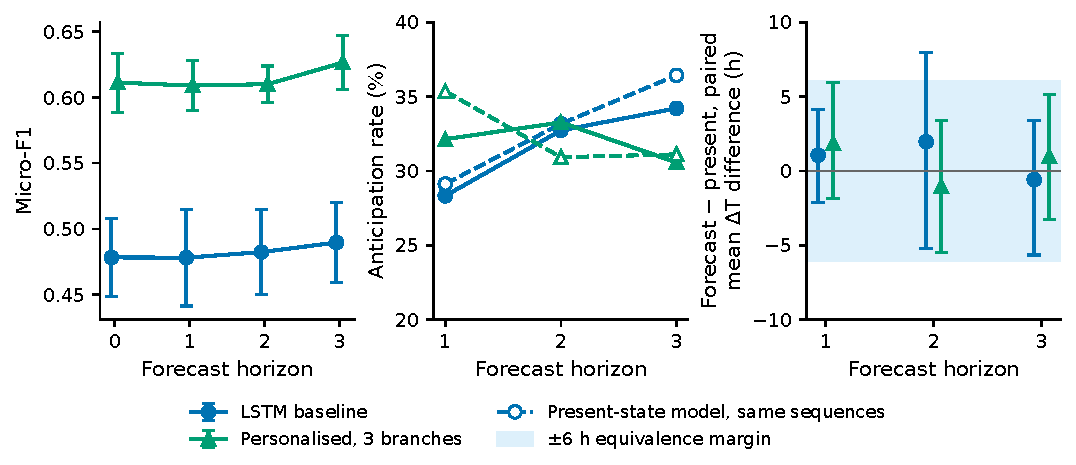
\includegraphics[width=\textwidth]{fig8_horizon.pdf}
\caption{Prediction-horizon experiment. Left: micro-F1 (error bars one
SD across folds). Centre: anticipation rate of the forecast-trained
model (solid) and of the present-state model on the same validation
sequences (dashed, open markers). Right: onset-paired mean \dt{}
difference, forecast minus present, with 95\% student-bootstrap
intervals against the $\pm 6$-hour margin. The horizon is the number of
EMA responses ahead that the model was trained to predict.}
\label{fig:horizon}
\end{figure}

Three results follow (Tables~\ref{tab:horizon},
\ref{tab:horizonnull} and~\ref{tab:horizondiff},
Figure~\ref{fig:horizon}).

First, against the expectation that forecasting is harder than
nowcasting, micro-F1 does not decay with horizon. It is flat to
slightly rising (0.478 to 0.490 for the baseline; 0.611 to 0.626 for
the three-branch model at a 49-hour median gap). Self-reported stress
is autocorrelated enough that predicting the label two days ahead is as
easy as predicting today's, which suggests the models track a
slow-moving person-level signal more than transition dynamics.

Second, a direct comparison of the horizon runs with the $h = 0$ runs
is misleading, and we report it because it misled us. Read down
Table~\ref{tab:horizonnull}, the mean \dt{} falls by 3 to 6 hours and the
anticipation rate rises by 4 to 11 points as the horizon grows, in all
six runs, and with students resampled jointly the 95\% interval for the
fall in mean \dt{} excludes zero in five of them. But the horizon runs
are validated on different sequences from the $h = 0$ runs: the last
examples of each student are dropped and the folds are stratified on
the shifted labels. The random-change-point null for those sequences
already shows the problem, since its anticipation rate rises by 2 to 5
points over the same horizons with no model involved.

Third, on identical sequences the apparent shift is not reproduced.
Every example has an out-of-fold prediction from the present-state
model of the same repetition, so for each validation sequence of a
forecast run we rebuilt the present-state model's trajectory on exactly
the same examples and compared the two onset by onset
(Table~\ref{tab:horizondiff}). The paired mean differences are between
$-1.0$ and $+2.0$ hours, with no consistent sign, and every 95\%
interval includes zero. The 90\% interval lies inside the $\pm 6$-hour
margin in five of the six runs; the exception is the baseline at
$h = 2$, whose interval reaches $+7.1$ hours. The anticipation rates of
the two models on the same sequences differ by at most 3.2 points,
again with every interval including zero, and each forecast run's mean
\dt{} lies inside the random-change-point null interval for its own
sequences. The present-state model, placed on the forecast runs'
sequences, shows the same lower mean \dt{} and higher anticipation rate
that the forecast-trained model does.

On identical validation sequences, no statistically detectable paired mean timing difference was found.
Equivalence within $\pm 6$ hours was supported for five of six comparisons; the baseline at $h = 2$ remained inconclusive.
We therefore have no evidence that training the models to forecast up
to 49 hours ahead moved their timing, and for one comparison we cannot
exclude a difference of up to 7 hours. What moved the statistics in the
direct comparison was the composition of the
evaluation sequences, which is a caution in its own right: \dt{}
summaries from different validation sequences are not comparable, even
for the same students and the same model, and comparisons should be
made on identical sequences, as the main analysis does. One caveat
applies to the same-sequence comparison: within a sequence, the
present-state predictions come from the five fold-models of one
repetition, each out-of-fold for its own examples, and not from a
single model.

\subsection{Sensitivity to the penalty and the matching window}
\label{sec:grid}

All results above fix the PELT penalty at 1.0 and the matching window
at 72 hours. Figure~\ref{fig:grid} repeats the main analysis over the
full grid penalty $\in \{0.5, 1, 2\}$ $\times$ window
$\in \{24, 48, 72, 96\}$ hours. The anticipation rate stays within
21--28\% in every cell with penalty $\leq 1$, rises mechanically with
the window (more distant matches admit more negatives and positives
alike), and is noisier at penalty 2, where the three-branch model
retains as few as 152 pairs. At penalty 5 fewer than a dozen pairs
survive per configuration and no estimate is meaningful; those cells
are listed in \ref{app:grid} for completeness. The median \dt{} is 0
hours in \emph{every} cell of the grid, and the ordering of the three
configurations is not stable across cells --- no choice of penalty or
window produces a personalisation advantage in timing.

\begin{figure}[htbp]
\centering
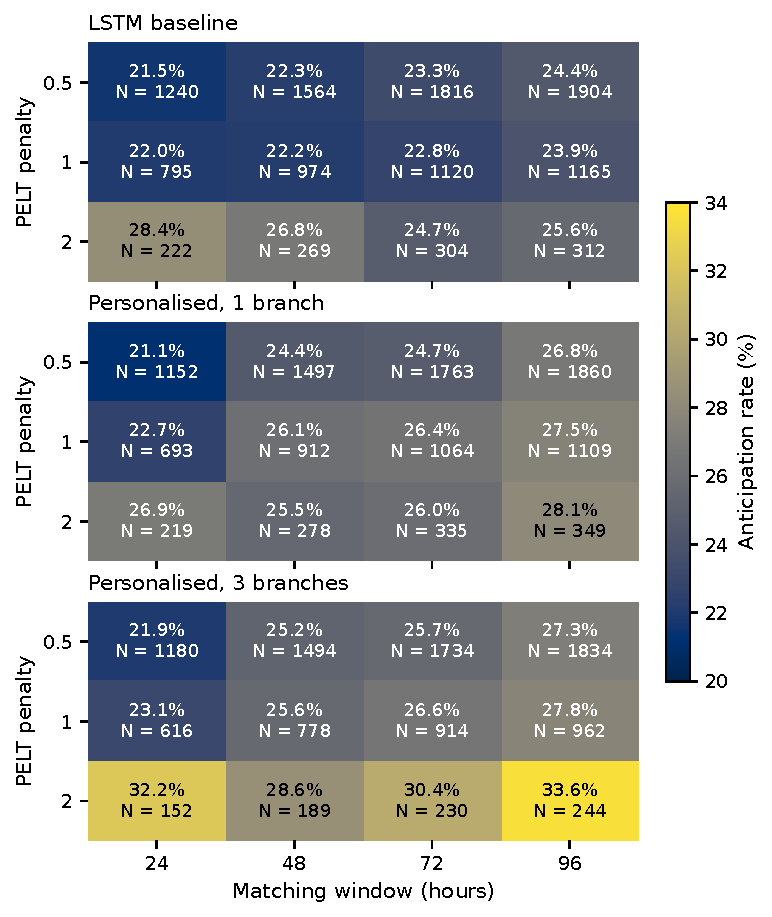
\includegraphics[width=0.8\textwidth]{fig9_sensitivity.pdf}
\caption{Anticipation rate over the PELT penalty $\times$ matching
window grid, with the number of matched pairs in each cell. The median
\dt{} is 0 hours in every cell. Penalty 5 (not shown) leaves fewer than
a dozen pairs per configuration.}
\label{fig:grid}
\end{figure}

%% ──────────────────────────────────────────────────────────────────────────
\section{Discussion}
%% ──────────────────────────────────────────────────────────────────────────

\subsection{Interpretation}

Four interventions were applied: single-branch personalisation,
three-branch personalisation, a timing-targeted training objective, and
retraining the models to forecast one to three EMA responses ahead. All
four left the median \dt{} at 0 hours. For the two personalisation
variants and the timing-targeted objective, the paired mean \dt{}
difference from the baseline is within the $\pm 6$-hour margin under a
student-level bootstrap. For the forecasting runs, compared with the
present-state models on identical sequences, the paired mean difference
is between $-1.0$ and $+2.0$ hours with every interval including zero,
and within the margin in five of six runs (the baseline at $h = 2$ is
the exception, so equivalence is not established there). The null
models show
that none of the main configurations has significantly more
anticipation than chance placement of change points, and that no
forecasting run does after correction for multiple tests; the baseline does show onset alignment
above the random-change-point null, so its change points are not
unrelated to the onsets, but they fall at or after them.

The most direct reading is that \dt{} measures a property of the data
and the annotation protocol rather than a property of the model. The
gap between when behavioural sensor signals shift and when a person
reports feeling stressed appears to be set by the sensing modality and
the ecological momentary assessment schedule, not by the model applied
to them.

This reading should be held with appropriate caution. What we
demonstrate is a bounded null across a specific family of models on a
single dataset: the paired analysis rules out between-model shifts
larger than 4.5 hours, but smaller shifts remain possible, and other
model families might behave differently.

\subsection{Implications for system design}

For anyone building a stress-monitoring system intended to support
intervention, the implication is direct. In this dataset the
anticipation rate sits between 23\% and 27\% for the baseline, both
personalised models, and both strengths of the timing-targeted
objective, and the null models show that this is not significantly
more than chance placement of change points produces under the same
matching rule. We find no evidence that any of these systems provides
early warning. Improving the classifier by 13.3 points of micro-F1 and
retargeting the loss produced no measurable shift in mean or median
timing. For retraining to forecast up to 49 hours ahead, no
statistically detectable paired mean timing difference was found on
identical validation sequences; equivalence within $\pm 6$ hours was
supported for five of six comparisons, and the baseline at $h = 2$
remained inconclusive.

This should be surprising to anyone who assumes accuracy and timeliness
improve together, and it is invisible to standard evaluation. We suggest
that studies reporting stress-prediction systems intended for
intervention include a timing measurement alongside classification
metrics. The \dt{} framework makes this possible without changes to the
model or additional annotation.

\subsection{Limitations}
\label{sec:limits}

\paragraph{Shared fold assignments} The ten repetitions use identical
deterministic fold assignments. The same subjects, onsets, and
trajectories appear in every repetition, with only model initialisation
differing. This tests whether architecture moves \dt{} with the data
held constant. It does not establish cohort-level generality, and the
effective number of independent observations is smaller than the raw
sample sizes suggest.

\paragraph{Statistical power} The paired equivalence analysis makes
the power explicit: between-model shifts are bounded within 4.5, 3.3,
and 2.8 hours for the three pairs at the 90\% level. A real
improvement smaller than these margins --- say two hours --- would not
be detected. The result should be read as a bounded null rather than a
demonstration of no effect.

\paragraph{Single cohort for the invariance test} The invariance test
proper derives from 23 students over one academic term (StudentLife).
Each subject contributes between zero and three matched pairs per fold.

\paragraph{Retrospective change points} PELT and the dynamic-programming
segmentation are offline procedures: each change point is located
using the subject's whole validation trajectory, including examples
after it. A negative \dt{} therefore means that the model's trajectory,
viewed in retrospect, changed before the reported onset. It does not
mean that a deployed system could have raised an alert at that time,
since an online detector needs evidence after the change to declare
it. \dt{} as measured here is at best an optimistic estimate of what
an online version could achieve, and measuring real-time warning lead would require an
online detector with an explicit detection delay.

\paragraph{Dependence on the evaluation sequence} The \dt{} summaries
depend on which examples make up a validation sequence. The same
present-state models give a mean \dt{} of $+6.7$ to $+8.4$ hours on
their own folds and $+0.7$ to $+4.0$ hours on the forecast runs' folds
(Section~\ref{sec:horizon}). Every comparison we draw conclusions from
is made on identical sequences, but absolute values of the mean \dt{}
and of the anticipation rate should not be compared across studies, or
across splits, without that control. In the same-sequence comparison
for the forecasting runs, the present-state predictions within a
sequence come from five fold-models and not one, the runs have five
repetitions each, and the $p$ values in Table~\ref{tab:horizonnull} are
uncorrected for six tests.

\paragraph{Heuristic matching rule} The 72-hour matching window and
nearest-neighbour rule were selected for this study. Different choices
produce different \dt{} distributions; Section~\ref{sec:grid} shows how
far the summary statistics move across four windows and three
penalties.

\paragraph{Temporal resolution} \dt{} is computed on each student's
validation subsequence within a fold, about ten EMA responses spread
over the term, so consecutive points are typically a day or more apart.
A third of matched pairs have $\Delta T = 0$ exactly because the change
point falls on the onset example itself. The metric cannot resolve
lead or lag finer than the spacing between responses, and a denser
evaluation sequence (for example a chronological hold-out) would give a
sharper measurement.

\paragraph{Withdrawn cross-modal analysis} The originally submitted
version included a \dt{} analysis of the WESAD wearable dataset. While
preparing this revision we found that the reference WESAD pipeline
evaluates with a shuffled data loader and stores no window index, so
the trajectories analysed there were not in temporal order and the
reported WESAD \dt{} values were not valid timing measurements. We have
withdrawn that analysis. All claims in this paper now rest on
StudentLife alone, and whether the result holds for physiological
wearable sensing is an open question.

\subsection{Future directions}

The immediate priority is a cross-modal test on physiological
wearable data, with the evaluation sequence kept in temporal order.
Beyond that, extending \dt{} to
a dataset with independent subject cohorts would address the shared-fold
limitation directly. Finally, the structural problem here --- detecting
a latent state transition before it becomes externally observable ---
is not specific to stress; the same measurement applies to any domain
where an early warning system is the goal. A companion paper transfers
the framework to mobile network signal quality prediction, providing
early evidence that the finding generalises beyond health sensing.

%% ──────────────────────────────────────────────────────────────────────────
\section{Conclusion}
%% ──────────────────────────────────────────────────────────────────────────

We introduced \dt{}, a measurement of when a stress-prediction model
detects a transition relative to when the person reports it, and showed
that its central tendency does not respond to the addition of
personalisation or to a training objective designed specifically to
move it. Retraining the models to forecast up to 49 hours ahead left
their accuracy unchanged; on identical validation sequences no
statistically detectable paired mean timing difference was found, with
equivalence within $\pm 6$ hours supported for five of six comparisons
and the baseline at $h = 2$ inconclusive. Across three configurations spanning 13.3 points of
micro-F1 on StudentLife, paired mean \dt{} differences on onsets
matched in both models fall within a $\pm 6$-hour equivalence margin,
no configuration shows significantly more anticipation than either of
two chance-level null models, and the median \dt{} is 0 hours under
every segmentation setting we tried. These are retrospective alignment
measurements, not real-time warning leads.

Timing and accuracy are separable properties of a stress-prediction
model. Standard evaluation metrics measure accuracy and are silent about
timing. Systems intended to anticipate stress rather than
merely recognise it will require methods that target timing directly,
and evaluation protocols that measure whether they succeed.

%% ──────────────────────────────────────────────────────────────────────────
\section*{CRediT authorship contribution statement}
%% ──────────────────────────────────────────────────────────────────────────

\textbf{David Olutunde Daniel:} Conceptualization, Methodology,
Software, Validation, Formal analysis, Investigation, Data curation,
Writing -- original draft, Writing -- review and editing, Visualization.

%% ──────────────────────────────────────────────────────────────────────────
\section*{Declaration of competing interest}
%% ──────────────────────────────────────────────────────────────────────────

The author declares no known competing financial interests or personal
relationships that could have appeared to influence the work reported in
this paper. The research was conducted during a research internship at
AT\&T, funded through Tech Mahindra (Americas) Inc.

%% ──────────────────────────────────────────────────────────────────────────
\section*{Ethics statement}
%% ──────────────────────────────────────────────────────────────────────────

This study is a secondary computational analysis of publicly available,
de-identified datasets collected and released by their original
investigators. No new data collection involving human participants was
undertaken, and no personally identifying information was accessed.
Additional institutional review board approval was therefore not
required.

%% ──────────────────────────────────────────────────────────────────────────
\section*{Data availability}
%% ──────────────────────────────────────────────────────────────────────────

The StudentLife dataset is publicly available from Dartmouth College.
The reference implementation and its preprocessed
data assets are distributed through the public repository cited in the
references \citep{iflrepo}. Analysis scripts supporting the \dt{}
framework, the tables of matched pairs underlying every result, and
the figures in this paper are available from the corresponding author
on reasonable request.

%% ──────────────────────────────────────────────────────────────────────────
\section*{Declaration of generative AI and AI-assisted technologies in
the writing process}
%% ──────────────────────────────────────────────────────────────────────────

During the preparation of this work the author used a generative AI
assistant solely to improve the clarity, readability, and language of the
manuscript text. After using this tool the author reviewed and edited
the content as needed and takes full responsibility for the content of
the publication. All experimental design, code, data processing,
numerical results, figures, and scientific conclusions were produced and
verified independently by the author. No AI-generated text was included
without human review.

%% ──────────────────────────────────────────────────────────────────────────
\section*{Acknowledgments}
%% ──────────────────────────────────────────────────────────────────────────

This research was conducted during a summer research internship at
AT\&T, funded through Tech Mahindra (Americas) Inc. The author thanks
the AT\&T Research team for providing the H100 GPU infrastructure that
supported the original experiments. The experiments for the revised
version were run on the Juno high-performance computing cluster at The
University of Texas at Dallas. The StudentLife dataset is made
available by its original investigators at Dartmouth College and is
gratefully acknowledged.

\appendix
\section{Sensitivity to the trajectory definition}
\label{app:maxprob}

Table~\ref{tab:traj} repeats the main analysis under three trajectory
definitions at \texttt{jump}~$=1$ --- the expected stress level of
Eq.~\ref{eq:stress} (main text), the maximum class probability used in
the originally submitted version, and the high-stress class probability
$p_t^{(2)}$ --- and, for completeness, under the originally submitted
configuration (maximum probability with the \texttt{ruptures} default
candidate grid of every fifth sample). These are descriptive sensitivity results; no equivalence test was
run on them. The pattern is the same under every definition: anticipation rates stay within
22--27\%, and the medians are 0 hours for every \texttt{jump}~$=1$
analysis. The submitted configuration shows how the coarse candidate
grid shrinks the number of matched pairs by roughly a factor of three
and inflates the medians to $+4.0$ to $+5.5$ hours, which accounts for
the differences between the originally submitted tables and those in
this revision.

\begin{table}[h]
\centering
\caption{\dt{} under alternative trajectory definitions. Anticipation
is the repetition mean $\pm$ SD. All analyses use PELT with penalty 1.0
and the 72-hour window.}
\label{tab:traj}
\small
\resizebox{\textwidth}{!}{%
\begin{tabular}{llcccc}
\toprule
Trajectory & Configuration & $N$ & Mean (h) & Median (h) & Anticipation \\
\midrule
\multirow{3}{*}{Expected stress, $s_t$ (main text)}
 & LSTM baseline       & 1120 & $+8.40$  & 0 & $22.8 \pm 2.1$\% \\
 & Personalised, 1 br. & 1064 & $+6.97$  & 0 & $26.4 \pm 2.7$\% \\
 & Personalised, 3 br. & 914  & $+6.65$  & 0 & $26.7 \pm 4.8$\% \\
\midrule
\multirow{3}{*}{Maximum probability}
 & LSTM baseline       & 965  & $+6.81$  & 0 & $24.0 \pm 4.4$\% \\
 & Personalised, 1 br. & 1073 & $+7.71$  & 0 & $25.9 \pm 3.8$\% \\
 & Personalised, 3 br. & 946  & $+8.69$  & 0 & $24.1 \pm 5.4$\% \\
\midrule
\multirow{3}{*}{$P(\text{high stress})$, $p_t^{(2)}$}
 & LSTM baseline       & 1056 & $+10.32$ & 0 & $22.2 \pm 2.8$\% \\
 & Personalised, 1 br. & 1092 & $+7.09$  & 0 & $25.8 \pm 2.0$\% \\
 & Personalised, 3 br. & 932  & $+8.06$  & 0 & $25.8 \pm 2.2$\% \\
\midrule
\multirow{3}{*}{Max.\ probability, default grid (as submitted)}
 & LSTM baseline       & 332  & $+11.05$ & $+4.0$ & $24.7 \pm 5.8$\% \\
 & Personalised, 1 br. & 420  & $+13.69$ & $+5.5$ & $24.7 \pm 3.5$\% \\
 & Personalised, 3 br. & 358  & $+15.78$ & $+5.5$ & $23.7 \pm 4.0$\% \\
\bottomrule
\end{tabular}}
\end{table}


\section{Full penalty and matching-window grid}
\label{app:grid}

Table~\ref{tab:grid} lists every cell of the sensitivity grid of
Section~\ref{sec:grid}, including penalty 5, where too few matched
pairs remain for the rates to be meaningful. The median \dt{} is 0
hours in every cell.

\begin{table}[h]
\centering
\caption{Anticipation rate, with the number of matched pairs in
parentheses, for every PELT penalty and matching window.}
\label{tab:grid}
\small
\begin{tabular}{ccccc}
\toprule
Penalty & Window (h) & LSTM baseline & Personalised, 1 br. & Personalised, 3 br. \\
\midrule
\multirow{4}{*}{0.5} & 24 & 21.5\% (1240) & 21.1\% (1152) & 21.9\% (1180) \\
 & 48 & 22.3\% (1564) & 24.4\% (1497) & 25.2\% (1494) \\
 & 72 & 23.3\% (1816) & 24.7\% (1763) & 25.7\% (1734) \\
 & 96 & 24.4\% (1904) & 26.8\% (1860) & 27.3\% (1834) \\
\midrule
\multirow{4}{*}{1} & 24 & 22.0\% (795) & 22.7\% (693) & 23.1\% (616) \\
 & 48 & 22.2\% (974) & 26.1\% (912) & 25.6\% (778) \\
 & 72 & 22.8\% (1120) & 26.4\% (1064) & 26.6\% (914) \\
 & 96 & 23.9\% (1165) & 27.5\% (1109) & 27.8\% (962) \\
\midrule
\multirow{4}{*}{2} & 24 & 28.4\% (222) & 26.9\% (219) & 32.2\% (152) \\
 & 48 & 26.8\% (269) & 25.5\% (278) & 28.6\% (189) \\
 & 72 & 24.7\% (304) & 26.0\% (335) & 30.4\% (230) \\
 & 96 & 25.6\% (312) & 28.1\% (349) & 33.6\% (244) \\
\midrule
\multirow{4}{*}{5} & 24 & 30.0\% (10) & 25.0\% (8) & 33.3\% (6) \\
 & 48 & 30.0\% (10) & 25.0\% (8) & 25.0\% (8) \\
 & 72 & 30.0\% (10) & 20.0\% (10) & 18.2\% (11) \\
 & 96 & 30.0\% (10) & 20.0\% (10) & 18.2\% (11) \\
\bottomrule
\end{tabular}
\end{table}

\newpage
%% ──────────────────────────────────────────────────────────────────────────
\bibliographystyle{elsarticle-harv}
\begin{thebibliography}{99}

\bibitem[Bakker et al.(2011)]{bakker2011}
Bakker, J., Pechenizkiy, M., Sidorova, N., 2011.
What's your current stress level? Detection of stress patterns from
GSR sensor data.
Proceedings of the 2011 IEEE 11th International Conference on Data
Mining Workshops, 573--580.
\url{https://doi.org/10.1109/ICDMW.2011.178}.

\bibitem[Beam and Kohane(2018)]{beam2018}
Beam, A.L., Kohane, I.S., 2018.
Big data and machine learning in health care.
JAMA 319, 1317--1318.
\url{https://doi.org/10.1001/jama.2017.18391}.

\bibitem[Chrousos(2009)]{chrousos2009}
Chrousos, G.P., 2009.
Stress and disorders of the stress system.
Nature Reviews Endocrinology 5, 374--381.
\url{https://doi.org/10.1038/nrendo.2009.106}.

\bibitem[Cohen et al.(1983)]{cohen1983}
Cohen, S., Kamarck, T., Mermelstein, R., 1983.
A global measure of perceived stress.
Journal of Health and Social Behavior 24, 385--396.
\url{https://doi.org/10.2307/2136404}.

\bibitem[De Bois et al.(2022)]{debois2022}
De Bois, M., El Yacoubi, M.A., Ammi, M., 2022.
GLYFE: review and benchmark of personalized glucose predictive models in
type 1 diabetes.
Medical \& Biological Engineering \& Computing 60, 1--17.
\url{https://doi.org/10.1007/s11517-021-02437-4}.

\bibitem[Futoma et al.(2020)]{futoma2020}
Futoma, J., Simons, M., Panch, T., Doshi-Velez, F., Celi, L.A., 2020.
The myth of generalisability in clinical research and machine learning
in health care.
The Lancet Digital Health 2, e489--e492.
\url{https://doi.org/10.1016/S2589-7500(20)30186-2}.

\bibitem[Gjoreski et al.(2017)]{gjoreski2016}
Gjoreski, M., Lu\v{s}trek, M., Gams, M., Gjoreski, H., 2017.
Monitoring stress with a wrist device using context.
Journal of Biomedical Informatics 73, 159--170.
\url{https://doi.org/10.1016/j.jbi.2017.08.006}.

\bibitem[Goldstein et al.(2017)]{goldstein2017}
Goldstein, B.A., Navar, A.M., Pencina, M.J., Ioannidis, J.P.A., 2017.
Opportunities and challenges in developing risk prediction models with
electronic health records data.
Journal of the American Medical Informatics Association 24, 198--208.
\url{https://doi.org/10.1093/jamia/ocw042}.

\bibitem[Henry et al.(2015)]{henry2015}
Henry, K.E., Hager, D.N., Pronovost, P.J., Saria, S., 2015.
A targeted real-time early warning score (TREWScore) for septic shock.
Science Translational Medicine 7, 299ra122.
\url{https://doi.org/10.1126/scitranslmed.aab3719}.

\bibitem[Hovsepian et al.(2015)]{hovsepian2015}
Hovsepian, K., al'Absi, M., Ertin, E., Kamarck, T., Nakajima, M.,
Kumar, S., 2015.
cStress: Towards a gold standard for continuous stress assessment in
the mobile environment.
Proceedings of the 2015 ACM International Joint Conference on Pervasive
and Ubiquitous Computing (UbiComp '15), 493--504.
\url{https://doi.org/10.1145/2750858.2807526}.

\bibitem[Information Fusion Lab(2021)]{iflrepo}
Information Fusion Lab, University of Massachusetts Amherst, 2021.
personalized-stress-prediction. GitHub repository.
\url{https://github.com/Information-Fusion-Lab-Umass/personalized-stress-prediction}.

\bibitem[Ebrahimzadeh et al.(2018)]{ebrahimzadeh2018}
Ebrahimzadeh, E., Kalantari, M., Joulani, M., Shahrokhi Shahraki, R.,
Fayaz, F., Ahmadi, F., 2018.
Prediction of paroxysmal atrial fibrillation: A machine learning based
approach using combined feature vector and mixture of expert
classification on HRV signal.
Computer Methods and Programs in Biomedicine 165, 53--67.
\url{https://doi.org/10.1016/j.cmpb.2018.07.014}.

\bibitem[Jackson et al.(2005)]{jackson2005}
Jackson, B., Scargle, J.D., Barnes, D., Arabhi, S., Alt, A.,
Gioumousis, P., Gwin, E., Sangtrakulcharoen, P., Tan, L., Tsai, T.T.,
2005.
An algorithm for optimal partitioning of data on an interval.
IEEE Signal Processing Letters 12, 105--108.
\url{https://doi.org/10.1109/LSP.2001.838216}.

\bibitem[Killick et al.(2012)]{killick2012}
Killick, R., Fearnhead, P., Eckley, I.A., 2012.
Optimal detection of changepoints with a linear computational cost.
Journal of the American Statistical Association 107, 1590--1598.
\url{https://doi.org/10.1080/01621459.2012.737745}.

\bibitem[Lei et al.(2018)]{lei2018}
Lei, Y., Li, N., Guo, L., Li, N., Yan, T., Lin, J., 2018.
Machinery health prognostics: A systematic review from data acquisition
to RUL prediction.
Mechanical Systems and Signal Processing 104, 799--834.
\url{https://doi.org/10.1016/j.ymssp.2017.11.016}.

\bibitem[McEwen(2007)]{mcewen2007}
McEwen, B.S., 2007.
Physiology and neurobiology of stress and adaptation: Central role of
the brain.
Physiological Reviews 87, 873--904.
\url{https://doi.org/10.1152/physrev.00041.2006}.

\bibitem[Pineau et al.(2021)]{pineau2021}
Pineau, J., Vincent-Lamarre, P., Sinha, K., Larivi\`{e}re, V.,
Beygelzimer, A., d'Alch\'{e}-Buc, F., Fox, E., Larochelle, H., 2021.
Improving reproducibility in machine learning research.
Journal of Machine Learning Research 22, 1--20.

\bibitem[Sano and Picard(2013)]{sano2013}
Sano, A., Picard, R.W., 2013.
Stress recognition using wearable sensors and mobile phones.
Proceedings of the 2013 Humaine Association Conference on Affective
Computing and Intelligent Interaction (ACII), 671--676.
\url{https://doi.org/10.1109/ACII.2013.117}.

\bibitem[Schmidt et al.(2018)]{schmidt2018}
Schmidt, P., Reiss, A., Duerichen, R., Marberger, C.,
Van Laerhoven, K., 2018.
Introducing WESAD, a multimodal dataset for wearable stress and affect
detection.
Proceedings of the 20th ACM International Conference on Multimodal
Interaction (ICMI '18), 400--408.
\url{https://doi.org/10.1145/3242969.3242985}.

\bibitem[Taylor et al.(2020)]{taylor2020}
Taylor, S., Jaques, N., Nosakhare, E., Sano, A., Picard, R., 2020.
Personalized multitask learning for predicting tomorrow's mood, stress,
and health.
IEEE Transactions on Affective Computing 11, 200--213.
\url{https://doi.org/10.1109/TAFFC.2017.2784832}.

\bibitem[Truong et al.(2020)]{truong2020}
Truong, C., Oudre, L., Vayatis, N., 2020.
Selective review of offline change point detection methods.
Signal Processing 167, 107299.
\url{https://doi.org/10.1016/j.sigpro.2019.107299}.

\bibitem[Wang et al.(2014)]{wang2014}
Wang, R., Chen, F., Chen, Z., Li, T., Harari, G., Tignor, S., Zhou,
X., Ben-Zeev, D., Campbell, A.T., 2014.
StudentLife: Assessing mental health, academic performance and behavioral
trends of college students using smartphones.
Proceedings of the 2014 ACM International Joint Conference on Pervasive
and Ubiquitous Computing (UbiComp '14), 3--14.
\url{https://doi.org/10.1145/2632048.2632054}.

\end{thebibliography}

\end{document}